
\documentclass{standalone}
\usepackage{tikz}
\usetikzlibrary{arrows.meta, positioning}

\usepackage{amssymb} 
\usetikzlibrary{shapes.geometric}
\newcommand\px{0}
\newcommand\ftf{6}
\newcommand\atf{12}
\begin{document}
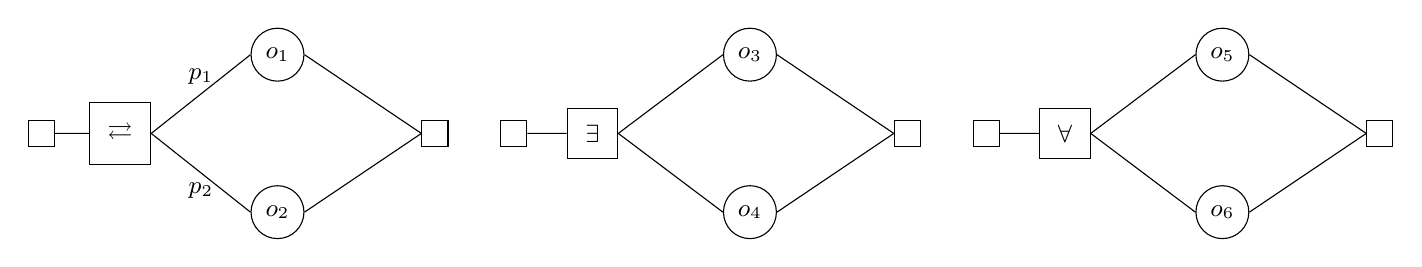
\begin{tikzpicture}[square/.style={regular polygon,regular polygon sides=4}]

    % Probability 
    \node at (\px, 0) [square, draw] (s) {}; 
    \node at (\px + 1, 0) [square, draw] (probab) {\small $\rightleftarrows$};
    \node at (\px + 3, 1) [circle, draw] (o3) {\small $o_1$};
    \node at (\px + 3, -1) [circle, draw] (o4) {\small $o_2$};
    \node at (\px + 5, 0) [square, draw] (e) {};

    \draw (s.east) -- (probab.west);
    \draw (probab.east) -- (o3.west) node[midway, above] {\small $p_1$};
    \draw (probab.east) -- (o4.west) node[midway, below] {\small $p_2$};
    \draw (o3.east) -- (e.west);
    \draw (o4.east) -- (e.west);

    %Ftf

    \node at (\ftf, 0) [square, draw] (s_f) {}; 
    \node at (\ftf + 1, 0) [square, draw] (ftf) {\small $\exists$};
    \node at (\ftf + 3, 1) [circle, draw] (o5) {\small $o_3$};
    \node at (\ftf + 3, -1) [circle, draw] (o6) {\small $o_4$};
    \node at (\ftf + 5, 0) [square, draw] (e_f) {};

    \draw (s_f.east) -- (ftf.west);
    \draw (ftf.east) -- (o5.west);
    \draw (ftf.east) -- (o6.west);
    \draw (o5.east) -- (e_f.west);
    \draw (o6.east) -- (e_f.west);

    %ATF
 
    \node at (\atf, 0) [square, draw] (s_a) {}; 
    \node at (\atf + 1, 0) [square, draw] (atf) {\small $\forall$};
    \node at (\atf + 3, 1) [circle, draw] (o7) {\small $o_5$};
    \node at (\atf + 3, -1) [circle, draw] (o8) {\small $o_6$};
    \node at (\atf + 5, 0) [square, draw] (e_a) {};

    \draw (s_a.east) -- (atf.west);
    \draw (atf.east) -- (o7.west);
    \draw (atf.east) -- (o8.west); 
    \draw (o7.east) -- (e_a.west);
    \draw (o8.east) -- (e_a.west);


\end{tikzpicture}
\end{document}
